\section{Power BI 组成架构}

Power BI由若干个应用服务组成,它们可互相协作工作。其中较为基础和常用的三个分别是:

\begin{enumerate}
    \item Power BI Desktop:桌面端的免费应用,专为分析人员设计,可用于连接、转换和可视化数据。 使用 Power BI Desktop,你可以连接到多个不同的数据源,并将它们(通常称为建模)组合成一个数据模型。 通过此数据模型,可以构建视觉对象以及可以作为报告与组织内的其他人共享的可视化对象集合。 大多数从事商业智能项目的用户使用 Power BI Desktop 创建报表,然后使用 Power BI service 与他人共享他们的报表。 
    \item Power BI service:在线SaaS服务。从Power BI Desktop中制作的报表发布后,就会显示在Power BI service中,用户可以在浏览器中查看、分享、发布Power BI报表,也可以设置数据刷新计划、管理数据的安全性等。其中,仪表板可帮助你掌握业务的脉搏。 仪表板以磁贴的形式显示,你可以选择这些磁贴打开报告以进一步查看详情。 仪表板和报告连接到数据集,将所有相关数据集中在一个地方。 
    \item Power BI Mobile:适用于Windows、安卓和iOS移动端APP。在移动端设备查看和跟踪数据时便可用到它,它让每一个人都获得触手可及的交互式数据报表。
\end{enumerate}

如\figref{fig:powerbi_3components}显示了这三者共同工作的界面图,它们正显示和处理了同一份数据,但有不同的UI,面向了不同的终端场景,能够让用户创造、分享、处理商业数据,让工作流更为高效。除这三者之外,Power BI的另外两个元素分别为Power BI 报表构建器(Report Builder)和Power BI 报表服务器(Report Server)。前者用于创建分页报表以在Power BI服务上共享。后者目前是一种本地报表服务器,可在Power BI Desktop中创建并发布,未来可灵活迁移到云。

\begin{figure}[htbp]
    \centering
    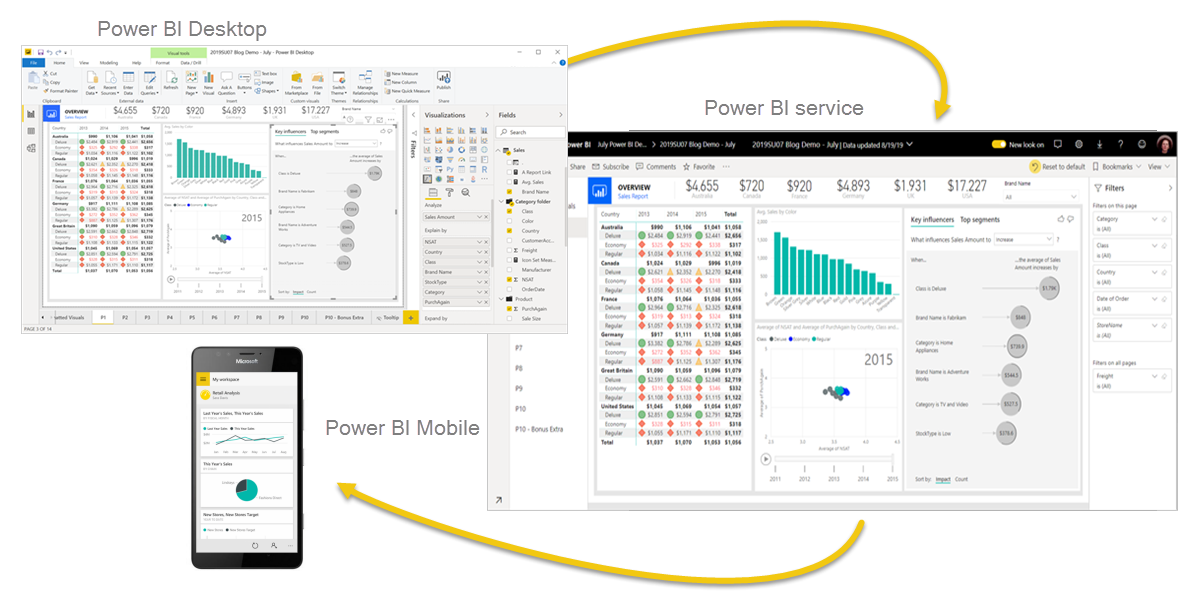
\includegraphics[width=0.9\textwidth]{figure/PowerBI/powerbi_3components.png}
    \caption{\textbf{Power BI Desktop、service和Mobile 三者协作}}
    \label{fig:powerbi_3components}
\end{figure}

由于数据处理和分析大部分的环节都在电脑上的桌面版完成,故本章节将主要介绍Power BI Desktop这款桌面端的应用,从案例出发介绍若干实际场景下的数据可视化的模块和具体操作。